\documentclass[a4j]{jarticle}
\usepackage[dvipdfmx]{graphicx}
\usepackage[dvipdfmx]{color}
\usepackage{url}
\usepackage{here}

\begin{document}

\section{ユーザインタフェース}
私、UI書きます
\subsection{画面詳細}
本システムが提供するアプリケーションの画面遷移及び画面の詳細について説明します。
\subsubsection{初期設定画面}
図\ref{honjo_setup}に、アプリを初めて起動した際に表示される初期設定画面を示します。
この画面はユーザに『ニックネーム(名前)の入力』・『居住地域の選択』を行ってもらうために表示されます。
入力が完了しないと次の画面に遷移することはできません。

図\ref{honjo_setup}に示す番号と対応させる形式で、以下にその役割を示します。

\begin{figure}[H]
    \begin{center}
    \resizebox{8cm}{!}{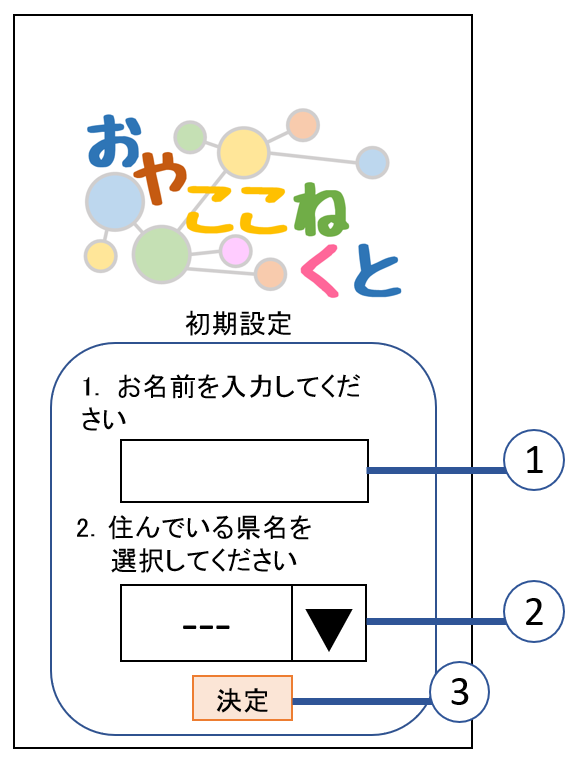
\includegraphics {honjo_FirstSetting.PNG}}
    \caption {初期設定画面}
    \label{honjo_setup}
    \end{center}
\end{figure}

\begin{enumerate}
  \renewcommand{\labelenumi}{\textcircled{\scriptsize \theenumi}}
  \item 名前(ニックネーム)の入力欄\\
        ユーザがアプリ内で使用したい名前を入力します。矩形領域をタップするとキーボードが開き、入力することが可能になります。
  \item 居住地域の選択欄\\
        ユーザの住んでいる地域を選択します。矩形領域をタップするとドロップダウンリストが開き、その中から住んでいる都道府県を選択します。
  \item 完了ボタン\\
        入力が完了したら押すボタンです。入力が正しくされている場合にのみメニュー画面(図\ref{honjo_main})へ遷移することができます。
\end{enumerate}


\subsubsection{メインメニュー画面}
図\ref{honjo_main}に、メインメニュー画面を示します。これは、アプリの初期設定を完了している場合に、最初に表示されます。
この画面は本アプリの持つ機能に遷移するために使用されます。

図\ref{honjo_main}に示す番号と対応させる形式で、以下にその役割を示します。

\begin{figure}[H]
    \begin{center}
    \resizebox{8cm}{!}{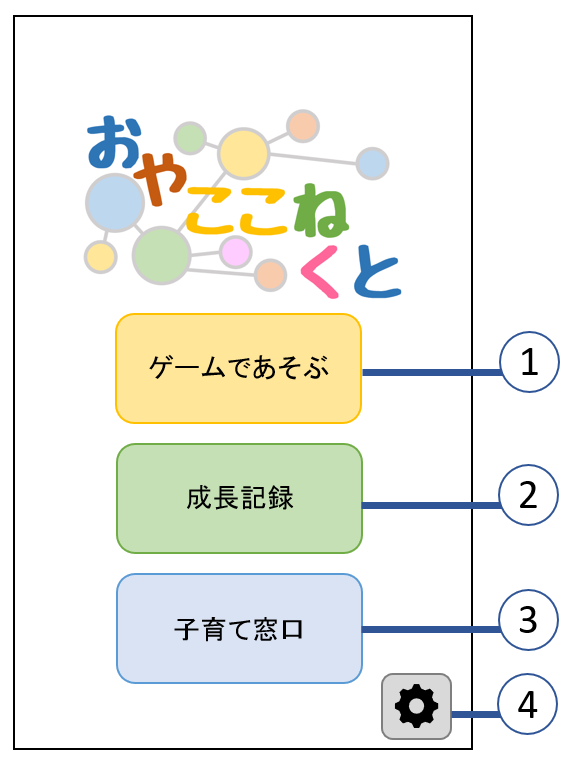
\includegraphics {honjo_main.PNG}}
    \caption {初期設定画面}
    \label{honjo_main}
    \end{center}
\end{figure}

\begin{enumerate}
  \renewcommand{\labelenumi}{\textcircled{\scriptsize \theenumi}}
  \item ゲーム画面遷移ボタン\\
        ゲーム機能を使用したい場合に押すボタンです。タップするとゲーム選択画面(図\ref{game})へ遷移します。
  \item 成長記録画面遷移ボタン\\
        成長記録機能を使用したい場合に押すボタンです。タップすると成長記録画面(図\ref{Grow})へ遷移します。
  \item 子育て窓口画面遷移ボタン\\
        子育て窓口機能を使用したい場合に押すボタンです。タップすると子育て窓口画面(図\ref{honjo_CR_Window})へ遷移します。
  \item 設定画面遷移ボタン\\
        アプリの設定を変更したい場合に押すボタンです。タップすると設定画面(図\ref{configration})へ遷移します。
\end{enumerate}


%%%%%%%%%%%%% 子育て窓口 %%%%%%%%%%%%%%%%%%%%%%%%%%%
%% CR = Child Raising = 子育て
\subsubsection{子育て窓口}
図\ref{honjo_CR_Window}に、子育て窓口の画面を示します。
子育てにおける不安・疑問を、検索や投稿を行うことによって解決するために使用されます。

図\ref{honjo_CR_Window}に示す番号と対応させる形式で、以下にその役割を示します。

\begin{figure}[H]
    \begin{center}
    \resizebox{8cm}{!}{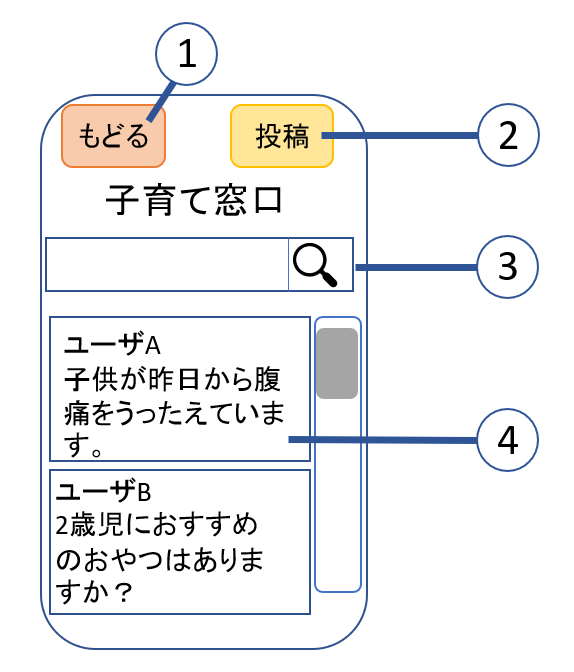
\includegraphics {honjo_CR_Window.PNG}}
    \caption {子育て窓口の画面}
    \label{honjo_CR_Window}
    \end{center}
\end{figure}

\begin{enumerate}
  \renewcommand{\labelenumi}{\textcircled{\scriptsize \theenumi}}
  \item 戻るボタン\\
        タップすると、メインメニュー画面(図\ref{honjo_main})へ遷移するボタンです。
  \item 質問投稿作成ボタン\\
        質問投稿をしたい時に押すボタンです。ペンのマークをタップすると、質問を行うための投稿画面(図\ref{honjo_CR_Contribution})へ遷移します。
  \item 質問の検索欄\\
        ユーザが子育て窓口内に投稿されたものを検索するために使用します。矩形領域をタップするとキーボードが開き、入力することが可能になります。
  \item 質問の一覧表示\\
        子育て窓口に投稿された質問が一覧表示されます。質問が書かれている矩形領域をタップすると質問の詳細画面(図\ref{honjo_CR_Answer})へ遷移します。
\end{enumerate}

\subsubsection{質問の詳細画面}
図\ref{honjo_CR_Answer}に、質問の詳細画面を示します。
質問の詳細を閲覧、またその質問に対して回答を行うために使用されます。

図\ref{honjo_CR_Answer}に示す番号と対応させる形式で、以下にその役割を示します。

\begin{figure}[H]
    \begin{center}
    \resizebox{8cm}{!}{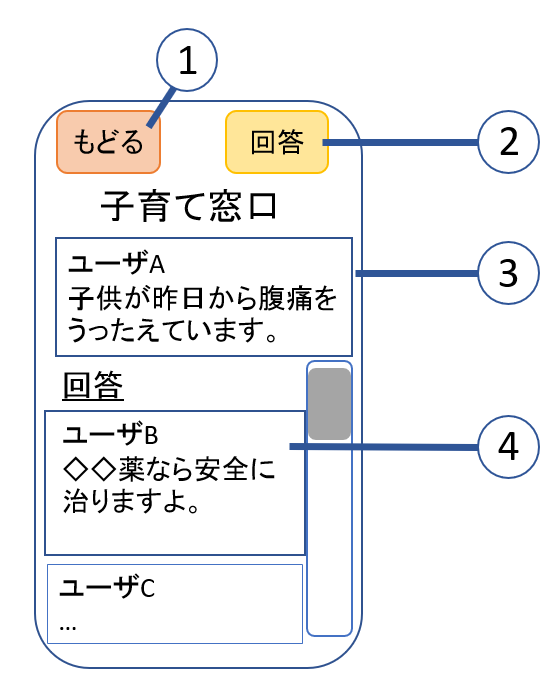
\includegraphics {honjo_CR_Answer.PNG}}
    \caption {質問の詳細画面}
    \label{honjo_CR_Answer}
    \end{center}
\end{figure}

\begin{enumerate}
  \renewcommand{\labelenumi}{\textcircled{\scriptsize \theenumi}}
  \item 戻るボタン\\
        タップすると、子育て窓口の画面へ遷移するボタンです。
  \item 回答ボタン\\
        この質問に対する回答を作成するためのボタンです。タップすると回答作成画面(図\ref{honjo_CR_CreateAnswer})へ遷移します。
  \item 質問内容\\
        質問内容の全文を表示します。
  \item 回答内容\\
        回答内容の全文を表示します。複数回答がある場合は下にスクロールすることで閲覧が可能になります。
\end{enumerate}


\subsubsection{回答作成画面}
図\ref{honjo_CR_CreateAnswer}に、回答の作成画面を示します。
ある質問に対する回答を行うために使用されます。

図\ref{honjo_CR_CreateAnswer}に示す番号と対応させる形式で、以下にその役割を示します。

\begin{figure}[H]
    \begin{center}
    \resizebox{8cm}{!}{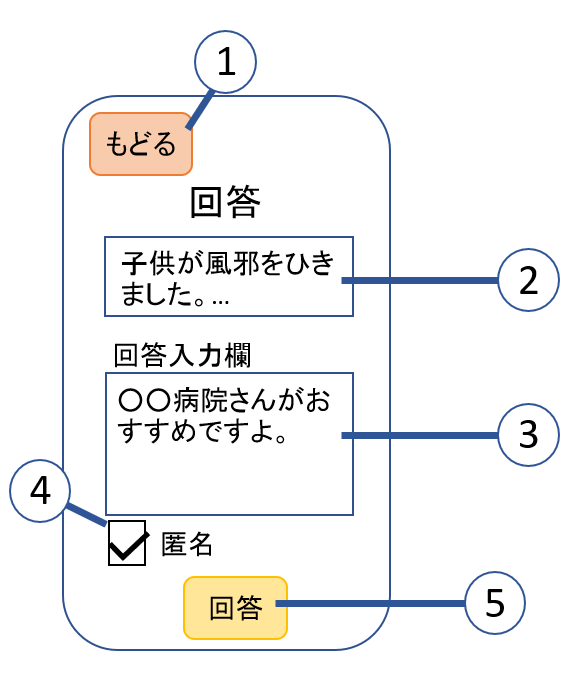
\includegraphics {honjo_CR_CreateAnswer.PNG}}
    \caption {回答作成画面}
    \label{honjo_CR_CreateAnswer}
    \end{center}
\end{figure}

\begin{enumerate}
  \renewcommand{\labelenumi}{\textcircled{\scriptsize \theenumi}}
  \item 戻るボタン\\
        タップすると、質問の詳細画面(図\ref{honjo_CR_Answer})へ遷移するボタンです。
  \item 質問内容\\
        質問内容の全文を表示します。
  \item 回答内容の入力欄\\
        ユーザが回答内容を入力するための欄です。矩形領域をタップするとキーボードが開き、入力することが可能になります。
  \item 匿名チェックボックス\\
        チェックボックスをタップして、チェックが入ると、匿名で回答を投稿することが出来ます。
  \item 回答投稿ボタン\\
        回答を入力欄に書き終えて投稿をしたい時に押すボタンです。回答投稿完了画面(図\ref{honjo_CR_CompleteAnswer})へ遷移します。
\end{enumerate}

\subsubsection{回答投稿完了画面}
図\ref{honjo_CR_CompleteAnswer}に、質問の投稿完了画面を示します。
質問の投稿が正常に完了したことを通知するために使用されます。

図\ref{honjo_CR_CompleteAnswer}に示す番号と対応させる形式で、以下にその役割を示します。

\begin{figure}[H]
    \begin{center}
    \resizebox{8cm}{!}{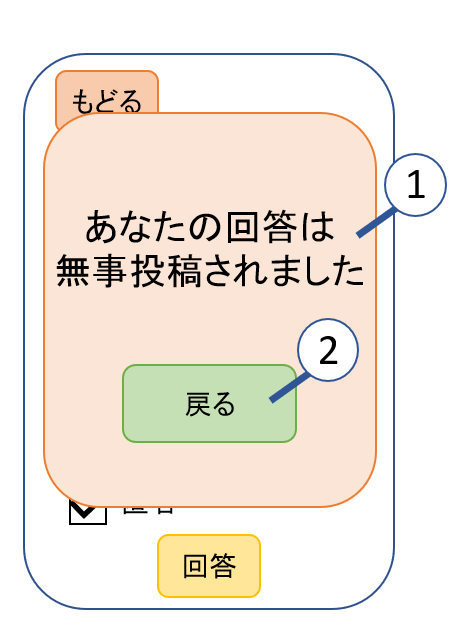
\includegraphics {honjo_CR_CompleteAnswer.PNG}}
    \caption {回答投稿画面}
    \label{honjo_CR_CompleteAnswer}
    \end{center}
\end{figure}

\begin{enumerate}
  \renewcommand{\labelenumi}{\textcircled{\scriptsize \theenumi}}
  \item ステータス\\
        ユーザの回答投稿が正常に完了したかを通知します。
  \item 戻るボタン\\
        子育て窓口の画面へ遷移するためのボタンです。
\end{enumerate}


\subsubsection{質問投稿画面}
図\ref{honjo_CR_Contribution}に、質問の投稿画面を示します。
質問の投稿を行うために使用されます。

図\ref{honjo_CR_Contribution}に示す番号と対応させる形式で、以下にその役割を示します。

\begin{figure}[H]
    \begin{center}
    \resizebox{8cm}{!}{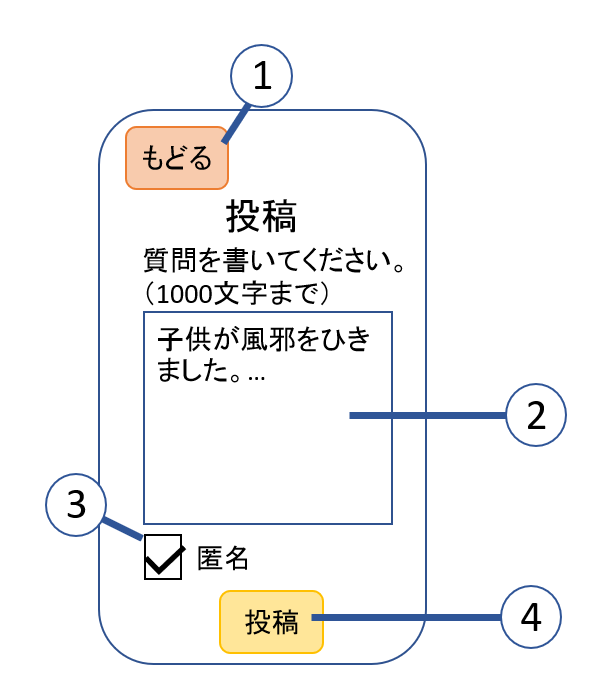
\includegraphics {honjo_CR_Contribution.PNG}}
    \caption {質問投稿画面}
    \label{honjo_CR_Contribution}
    \end{center}
\end{figure}

\begin{enumerate}
  \renewcommand{\labelenumi}{\textcircled{\scriptsize \theenumi}}
  \item 戻るボタン\\
        タップすると、子育て窓口の画面(図\ref{honjo_CR_Window})へ遷移するボタンです。
  \item 質問内容の入力欄\\
        ユーザが質問の内容を書き込むための欄です。矩形領域をタップするとキーボードが開き、入力することが可能になります。
  \item 匿名チェックボックス\\
        チェックボックスをタップして、チェックが入ると、匿名で回答を投稿することが出来ます。
  \item 投稿ボタン\\
        質問を入力欄に書き終えて投稿をしたい時に押すボタンです。質問投稿完了画面(図\ref{honjo_CR_CompleteContribution})へ遷移します。
\end{enumerate}

\subsubsection{質問投稿完了画面}
図\ref{honjo_CR_CompleteContribution}に、質問の投稿完了画面を示します。
質問の投稿が正常に完了したことを通知するために使用されます。

図\ref{honjo_CR_CompleteContribution}に示す番号と対応させる形式で、以下にその役割を示します。

\begin{figure}[H]
    \begin{center}
    \resizebox{8cm}{!}{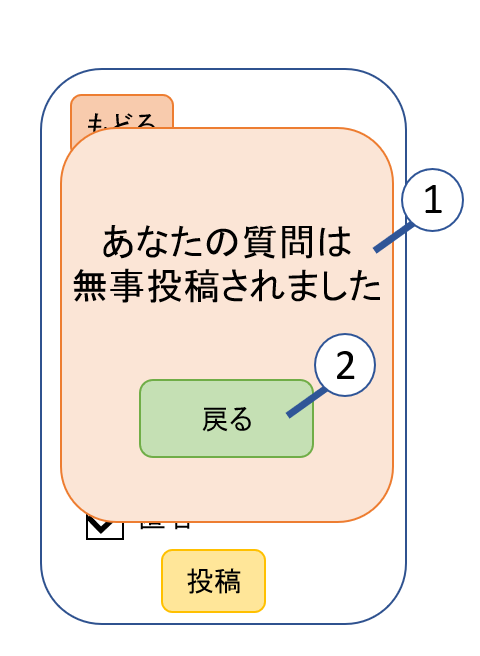
\includegraphics {honjo_CR_CompleteContribution.PNG}}
    \caption {質問投稿画面}
    \label{honjo_CR_CompleteContribution}
    \end{center}
\end{figure}

\begin{enumerate}
  \renewcommand{\labelenumi}{\textcircled{\scriptsize \theenumi}}
  \item ステータス\\
        ユーザの質問投稿が正常に完了したかを通知します。
  \item 戻るボタン\\
        子育て窓口の画面(図\ref{honjo_CR_Window})へ遷移するためのボタンです。
\end{enumerate}

\end{document}
